\documentclass[8pt]{beamer}

\usepackage[utf8]{inputenc}
\RequirePackage[francais]{babel}
%\usepackage{url}
%\usepackage{etex}
%\usepackage{enumitem}
\usepackage{multicol}
%\usepackage{bbm}
%\usepackage{amsmath,amsthm,amssymb}
%\usepackage[official]{eurosym}
%\usepackage{pifont}
%\usepackage{exercise}
%\usepackage{graphics}
%\usepackage{array,multirow,makecell}
%\usepackage{verbatim}
%\usepackage[dvipsnames]{pstricks}
\usepackage{pstricks-add,pst-plot,pst-text,pst-tree,pst-eps,pst-fill,pst-node,pst-math,pst-blur,pst-func}
%\usepackage{pgf,tikz}
%\usepackage{tipfr}
%\usepackage{thmbox}
%\usepackage{calc}
%\usepackage{ifthen}
%\usepackage{pdfpages}
%\usepackage{colortbl}
%\usepackage{sagetex}
%\usetikzlibrary{arrows,patterns}
%\input tabvar
%\usepackage{tkz-tab}
%\usepackage{listings}
%\usepackage[np]{numprint}
%\usepackage{fancybox,fancyhdr}
%\usepackage{thmtools}
%\usepackage{bclogo}
%\usepackage{lastpage}

\usepackage{tabularx}
\usepackage{array,multirow,makecell}
\usetheme{Madrid}
%\usetheme{Bergen}
\usecolortheme{beaver}
  
%----------------------------------------------------------------------------------------------- 
% 							Commandes Tableaux
%-----------------------------------------------------------------------------------------------
\setcellgapes{1pt}
\makegapedcells
\newcolumntype{R}[1]{>{\raggedleft\arraybackslash }b{#1}}
\newcolumntype{L}[1]{>{\raggedright\arraybackslash }b{#1}}
\newcolumntype{C}[1]{>{\centering\arraybackslash }b{#1}}

%\setbeamercolor

%Information to be included in the title page:
\title{Protocoles de routage}
\subtitle{RIP - OSPF}
\author{Yannick CHISTEL}
\institute{Lycée Dumont d'Urville - CAEN}
\date{\today}

\begin{document}
 
\frame{\titlepage}

\begin{frame}
\frametitle{Topologie d'un réseau}
\begin{block}{Définition}
Les routeurs sont des dispositifs qui permettent la communication entre les appareils terminaux se trouvant dans un réseau.
\begin{itemize}
\item On a les routeurs d'accès à un réseau dans lequel les machines sont reliées entre elles à l'aide de switchs eux-mêmes reliés au routeur.
\item On a les routeurs d'interconnexion de réseau, c'est à dire des routeurs reliés à d'autres routeurs  pour interconnecter différents réseaux.
\end{itemize}
On appelle topologie d'un réseau l'interconnexion de ces routeurs entre eux et les différents réseaux qu'ils relient.
\end{block}

\begin{block}{Adresse IP}
Le protocole IP (Internet Protocol) permet d'attribuer des adresses IPV 4 et/ou IPV 6 pour identifier chaque machine sur un réseau.

Une adresse IP se constitue de 2 parties : la \textbf{partie réseau} et la \textbf{partie qui identifie la machine}. Les valeurs qui identifient les machines sur un réseau sont délimités par le masque de réseau de la forme 255.255.255.0 (par exemple). Dans le masque, on a :
\begin{itemize}
\item Les valeurs 255 qui correspondent à l'adresse réseau ;
\item Les valeurs 0 qui indique la plage d'adresse disponible pour les machines.
\item On note, par exemple, l'adresse réseau et le masque sous la forme 192.168.1.0/24 qui correspond au masque 255.255.255.0
\end{itemize}
\end{block}

\end{frame}




\begin{frame}
\frametitle{Topologie d'un réseau}
\begin{exampleblock}{Exemple}
On considère la topologie réseau suivante: 6 routeurs et 2 réseaux locaux.\medskip

\begin{minipage}{3.8cm}
\textbf{1)~} Le réseau local a une adresse réseau de valeur 192.168.1.0/24.\smallskip

Cela signifie que le masque de réseau est 255.255.255.0 autorisant 255 adresses IP dont 1 est attribuée au routeur R1. \smallskip

Cela permet d'avoir jusqu'à 254 machines dans le réseau local.\bigskip

\textbf{2)~} L'adresse réseau entre les routeurs R1 et R3 a pour valeur 10.1.1.0/30.\smallskip

Le masque de réseau est 255.255.255.252 autorisant seulement 3 adresses IP. \smallskip
\end{minipage}\hfill
\begin{minipage}{8.2cm}
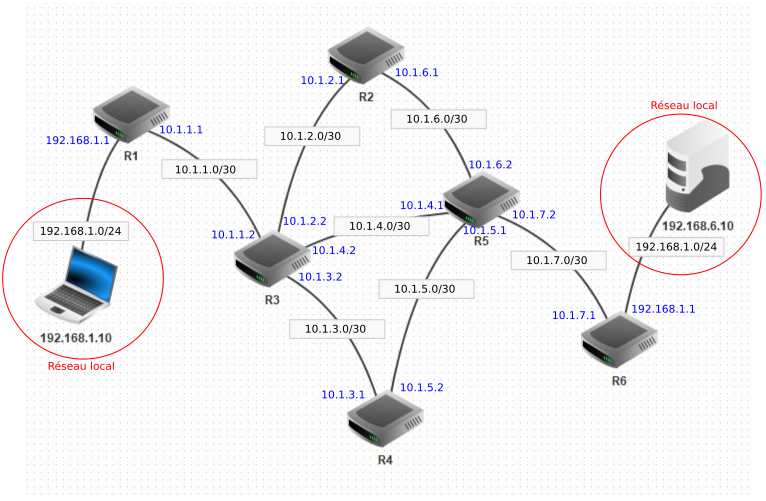
\includegraphics[scale=0.4]{img/topologie2.eps}
\end{minipage}
\end{exampleblock}
\end{frame}



\begin{frame}
\frametitle{Topologie d'un réseau}
\begin{block}{Définition}

On représente la topologie d'un réseau par un \textbf{graphe} dans lequel :
\begin{itemize}
\item Chaque \textbf{sommet} du graphe représente un routeur ou un réseau
\item Chaque arête du graphe représente une connexion entre 2 routeurs ou 2 réseaux.
\item Chaque poids (lorsqu'il est donné) représente le coût ou la distance entre 2 routeurs ou 2 réseaux.
\end{itemize}
\end{block}

\begin{exampleblock}{Exemple}
La topologie réseau de l'exemple précédent peut se représenter par le graphe.\medskip

\begin{minipage}{6cm}
Ici le \textbf{graphe} a 6 \textbf{sommets} et 7 \textbf{arêtes}.\medskip

Les \textbf{sommets} du graphe représentent les routeurs R1, R2, ..., R6.\medskip

Les \textbf{arêtes} représentes les liens entre les routeurs.
\end{minipage}\hfill
\begin{minipage}{6cm}
\begin{center}
\psset{unit=0.5cm}
\begin{pspicture}(10,6)
\cnodeput(0.5,3.5){R1}{R1}
\cnodeput(5.5,5.5){R2}{R2}
\cnodeput(2.5,3){R3}{R3}
\cnodeput(5,1){R4}{R4}
\cnodeput(7.5,3){R5}{R5}
\cnodeput(9.5,2.5){R6}{R6}
\ncline{R1}{R3}%\ncput*{\bf 2}
\ncline{R3}{R2}%\ncput*{\bf 4}
\ncline{R3}{R4}%\ncput*{\bf 6}
\ncline{R3}{R5}%\ncput*{\bf 5}
\ncline{R2}{R5}%\ncput*{\bf 2}
\ncline{R4}{R5}%\ncput*{\bf 1}
\ncline{R5}{R6}%\ncput*{\bf 5}
\end{pspicture}
\end{center} 
\end{minipage}
\end{exampleblock}

\end{frame}




\begin{frame}
\frametitle{Protocole de routage}


\begin{block}{Présentation}
Les routeurs utilisent un protocole pour communiquer entre eux, assurant ainsi l'acheminement des données entre les machines de deux réseaux distant.

Chaque routeur a une connaissance du réseau auquel il appartient. 

Ces données sont rassemblées dans une table de routage qui comprend notamment :
\begin{enumerate}
\item les adresses réseaux de destination avec lesquelles il peut communiquer;
\item les passerelles (routeurs) qui permettent d'accéder aux réseaux;
\item les interfaces réseaux sur lesquelles il faut envoyer les données.
\item les coûts pour optimiser l'acheminement des données : ce coût dépend du débit de la connexion ou du nombre de routeurs à traverser pour arriver à destination.
\end{enumerate}

Chaque machine contient aussi une table de routage qui mémorise les adresses réseaux avec lesquelles elles communiquent. Cette table peut être affichée avec la commande \textbf{arp}.
\end{block}

\begin{block}{Protocoles}
Il existe de nombreux protocoles de routage. On s'intéressera à deux protocoles qui sont RIP et OSPF.\smallskip

Les tables de routages sont régulièrement mises à jour grâce à des algorithmes:
\begin{itemize}
\item Le protocole RIP utilise l'algorithme de Bellman-Ford pour découvrir la topologie du réseau.
\item Le protocole OSPF utilise l'algorithme de Dijkstra pour déterminer la route la plus rapide
\end{itemize}
\end{block}

\end{frame}




\begin{frame}
\frametitle{Protocole RIP}

\begin{block}{Présentation}
Dans un réseau, chaque routeur dispose d'une table de routage qui contient les informations sur les routeurs avec lesquels il communique. \smallskip

Chaque routeur complète sa table de routage avec ses voisins immédiats. Il mémorise les réseaux directement reliés à lui, les interfaces utilisées puis met chaque distance à 1.\smallskip

Ensuite, il échange régulièrement sa table avec ses voisins et complète ou met à jour sa table de routage avec les informations détenues par les routeurs voisins.\smallskip

La table de routage d'un routeur se stabilise et dispose des informations sur tout le réseau.
\end{block}


\begin{exampleblock}{Exemple}
Table de routage du routeur R1 après avoir découvert la topologie du réseau (ci-dessus).
\begin{center}
\begin{tabular}{*{4}{|C{2.5cm}}|}\hline
\textbf{destination} & \textbf{passerelle} & \textbf{interface} & \textbf{distance}\\\hline
10.1.1.0/30& & eth0 & 1 \\\hline
192.168.1.0/24& & wlan0 & 1\\\hline
10.1.2.0/30& 10.1.1.2& eth0 & 2\\\hline
10.1.3.0/30& 10.1.1.2& eth0 & 2 \\\hline
10.1.4.0/30& 10.1.1.2& eth0 & 2\\\hline
10.1.7.0/30& 10.1.1.2& eth0 & 3 \\\hline
192.168.1.0/24& 10.1.1.2 & eth0 & 4 \\\hline
\end{tabular}
\end{center}
\end{exampleblock}
\end{frame}



\begin{frame}
\frametitle{Protocole RIP}

\begin{block}{Protocole RIP}
Un routeur qui reçoit les informations d'un routeur voisin suit les \textbf{4 règles du protocole RIP}:
\begin{enumerate}
\item il découvre une nouvelle route inconnue vers un sous réseau inconnu, il ajoute à sa table;
\item Il découvre une route plus courte vers un sous-réseau connu, mais passant par un nouveau routeur. L'ancienne route est remplacée par la nouvelle;
\item Il reçoit une nouvelle route plus longue vers un sous-réseau connu, il l'ignore;
\item Il reçoit une route plus longue vers un routeur passant par le même voisin, cela signifie qu'un problème est survenu sur l'ancienne route. Il met à jour sa table avec cette nouvelle route.
\end{enumerate}
Lorsqu'un routeur reçoit une route, il faut augmenter la distance de 1, soit pour la comparer aux autres routes, soit pour l'ajouter à sa table. Les distances indiquent le nombre de routeurs traversés pour accéder à un sous réseau. Lorsque la distance est supérieure à 15, la route est effacée de la table.
\end{block}

\begin{block}{Détection de panne}
Lorsqu'une panne survient sur le réseau, comme la rupture de communication entre 2 routeurs, les routeurs qui perdent la connexion envoient l'information aux autres routeurs avec un coût supérieur à 15 (en général 16) pour que les autres routeurs mettent à jour leurs tables. Il remplacent la route rompue par une autre route, certes plus longue que l'ancienne, mais qui permet d'acheminer les données.
\end{block}
\end{frame}

\begin{frame}
\frametitle{Protocole OSPF}

\begin{block}{Présentation}
Le protocole OSPF (Open Shortest Path First) est adapté pour de très grands réseaux. Les réseaux sont sont découpés en zones et le protocole OSPF gère chaque zone. Ensuite il gère le routage entre les zones. \medskip

La principale différence avec le protocole RIP est dans la prise en compte de la rapidité de transmission de l'information. L'algorithme de Dijkstra permet de déterminer la route la plus courte entre 2 routeurs. \medskip

Les routeurs échangent leurs informations et mettent à jour leurs tables de routage.

\begin{center}
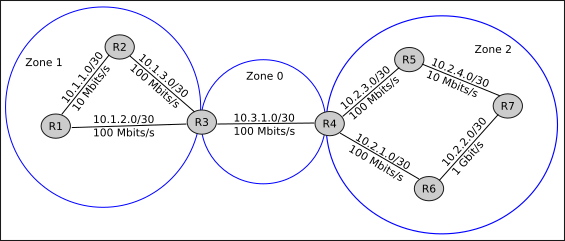
\includegraphics[scale=0.6]{img/ospf2.eps}
\end{center}
\end{block}
\end{frame}


\begin{frame}
\frametitle{Coût d'une liaison}

\begin{block}{Présentation}
Le protocole OSPF calcule le coût d'une liaison avec ses routeurs voisins. 

Le coût est fixé à $\dfrac{10^{8}}{d}$ où $d$ est le débit de la liaison donnée en bit par seconde (bit/s).

\end{block}
\begin{exampleblock}{Exemple}
Reprenons l'exemple précédent :
\begin{enumerate}
\item le \textbf{débit} entre le routeur R1 et R2 est de $10 \text{~Mbits/s~} = 10 \times 10^{6} \text{~bits/s~} = 10^{7} \text{~bits/s~}$.
\item Le \textbf{coût} est donc $\dfrac{10^{8}}{10^{7}}=10$
\end{enumerate}
On obtient le graphe suivant :
\begin{center}
\psset{unit=0.5cm}
\begin{pspicture}(10,6)
\cnodeput(0.5,3){R1}{R1}
\cnodeput(3,5.5){R2}{R2}
\cnodeput(4,3){R3}{R3}
\cnodeput(7,3){R4}{R4}
\cnodeput(7.5,5.5){R5}{R5}
\cnodeput(8,0.5){R6}{R6}
\cnodeput(9.5,3){R7}{R7}
\ncline{R1}{R3}\ncput*{1}
\ncline{R1}{R2}\ncput*{10}
\ncline{R3}{R2}\ncput*{1}
\ncline{R3}{R4}\ncput*{1}
\ncline{R4}{R5}\ncput*{1}
\ncline{R4}{R6}\ncput*{1}
\ncline{R5}{R7}\ncput*{10}
\ncline{R6}{R7}\ncput*{0,1}
\end{pspicture}
\end{center} 
\end{exampleblock}
\end{frame}



\begin{frame}
\frametitle{Algorithme de Dijkstra}

\begin{block}{Présentation}
L'algorithme de Dijkstra permet de déterminer la route la moins couteuse entre 2 routeurs.
\end{block}

\begin{exampleblock}{Exemple}
\begin{center}
\renewcommand\arraystretch{1.4}
\begin{tabular}{*{7}{|C{0.8cm}}|C{1.6cm}|}\hline 
R1 & R2 & R3 & R4 & R5 & R6 & R7 & Sommet fixé\\ \hline
$0$ & $\infty$ & $\infty$ & $\infty$ & $\infty$  & $\infty$ & $\infty$ & R1(0)\\ \hline
&$10_{R1}$&$1_{R1}$&$\infty$&$\infty$&$\infty$&$\infty$& R3(1)\\ \hline 
&$2_{R3}$&&$2_{R3}$&$\infty$&$\infty$&$\infty$&R2(2)\\ \hline 
&&&$2_{R3}$&$\infty$&$\infty$&$\infty$&R4(2)\\ \hline 
&&&&$3_{R4}$&$3_{R4}$&$\infty$&R5(3)\\ \hline 
&&&&&$3_{R4}$&$13_{R5}$&R6(3)\\ \hline 
&&&&&&$3,1_{R6}$&R7(3,1)\\ \hline 
\end{tabular}\medskip

La route la plus courte est donc $R1 \longmapsto R3 \longmapsto R4 \longmapsto R6 \longmapsto R7$ qui a un coût de $3,1$.
\end{center} 
\end{exampleblock}
\end{frame}


\end{document}

